\documentclass[pdflatex,sn-mathphys-num]{sn-jnl}

\usepackage{amsmath,amssymb,amsthm}
\usepackage{booktabs,array,tabularx,graphicx}
\usepackage{microtype}

\theoremstyle{thmstyleone}
\newtheorem{theorem}{Theorem}[section]
\newtheorem{proposition}[theorem]{Proposition}
\newtheorem{corollary}[theorem]{Corollary}
\theoremstyle{thmstyletwo}
\newtheorem{remark}[theorem]{Remark}

\newcommand{\Z}{\mathbb Z}
\newcommand{\TV}{\mathsf{TV}}
\newcommand{\Unif}{\mathsf{U}}
\newcommand{\rank}{\operatorname{rank}}
\newcommand{\E}{\mathbb E}
\newcommand{\Geom}{\mathsf{Geom}}
\newcommand{\HighBits}{\mathsf{HighBits}}
\newcommand{\woneEncode}{\mathsf{w1Encode}}

\title[Online Resource: rejection-sampling interfaces]{Online Resource 1:
Freshness, Restart, and Public-Rank Details for Lee-Shell Rejection Sampling}

\author[1]{\fnm{Anonymous} \sur{Submission}}
\affil[1]{\orgname{Anonymized for review}}

\begin{document}

\abstract{This online resource contains the probabilistic and algebraic
interfaces used by the brief rejection-sampling application in the main
manuscript.  It states and proves classical fresh-query and adaptive-restart
bounds, records the corresponding scoped quantum-random-oracle statements,
and derives a public rank--bucket certificate for the ML-DSA commitment map.
None of these results is used in the proofs of the Lee-ball
cross-covariogram, majorization, stability, or radial-correlation theorems.}

\keywords{rejection sampling, random oracle, adaptive restart, rank certificate}

\maketitle

\section{Classical and quantum freshness and restart details}
\label{app:qrom-details}

This resource first states and proves the two classical interfaces cited in
the main manuscript.  It then supplies the adaptive-reprogramming
specialization of Grilo et al.~\cite{GHHM21}, the complete-instrument restart
hybrid, and the exact scope conventions used by the QROM statements.

\begin{theorem}[Fresh-query interface]
\label{thm:rom-freshness}
Let $\mathcal X$ and $\mathcal C$ be finite, let $S\subset\Z^d$ be finite,
let $g_\theta:S\to\mathcal X$, and let
$\phi_\theta:\mathcal C\to\Z^d$.  Suppose
\[
 \varnothing\ne T\subseteq
 \bigcap_{\theta,c}(S+\phi_\theta(c)),
 \qquad a=|T|/|S|.
\]
Let $Y\sim\Unif(S)$ and, after an arbitrary classical random-oracle table
$H:\mathcal X\to\mathcal C$ with queried domain $Q_H$, put
\[
 C=H(g_\theta(Y)),\qquad Z=Y+\phi_\theta(C).
\]
Put $\eta_\theta=\Pr[g_\theta(Y)\in Q_H]$ and assume
$\eta_\theta<a$.  If the trial accepts exactly when $Z\in T$, then
\begin{align}
 |\Pr[Z\in T]-a|&\le\eta_\theta,\\
 \TV\bigl(\mathcal L_\theta(C,Z\mid Z\in T),
       \Unif(\mathcal C)\otimes\Unif(T)\bigr)
 &\le\eta_\theta/a.                                \label{eq:compact-rom}
\end{align}
If $q_H=|Q_H|$ and every commitment fiber has size at most $M_\theta$, then
\begin{equation}
 \eta_\theta\le\min\{1,q_HM_\theta/|S|\}
 =\min\{1,q_H2^{-H_\infty(g_\theta(Y))}\}.          \label{eq:rom-fiber}
\end{equation}
The same conclusion holds after a random adaptive classical transcript by
conditioning and averaging its hit probability.
\end{theorem}

\begin{proof}[Proof of Theorem~\ref{thm:rom-freshness}]
Couple the real challenge to an independent uniform challenge.  They agree
unless $g_\theta(Y)$ is already in the table, an event of probability
$\eta_\theta$.  In the fresh game, every translated source contains $T$, so
acceptance is exactly $a$ and the accepted law is
$\Unif(\mathcal C)\otimes\Unif(T)$.  Restricting two laws at distance
$\eta_\theta$ to an event of ideal mass $a$ gives the factor $1/a$.
The fiber union bound proves~\eqref{eq:rom-fiber}.
\end{proof}

\begin{theorem}[Adaptive restart composition]
\label{thm:retry-composition}
Suppose the ideal accepted sublaw at every retry history is the same $aQ$,
while the real and ideal full-trial kernels at round $i$ couple with error at
most $e_i$.  Then the joint law of the stopping time and accepted output is
within
\begin{equation}
 \min\left\{1,\sum_{i\ge1}(1-a)^{i-1}e_i\right\}
 \label{eq:compact-retry}
\end{equation}
of $\Geom(a)\otimes Q$.  In particular, if each rejection adds one table
entry and the conditional commitment point mass is at most $2^{-h}$, the
classical error is at most
\begin{equation}
 2^{-h}\left(\frac{q_0}{a}+\frac{1-a}{a^2}\right).
 \label{eq:compact-growing-table}
\end{equation}
\end{theorem}

\begin{proof}[Proof of Theorem~\ref{thm:retry-composition}]
Charge the first coupling disagreement at round $i$.  The ideal process
reaches that round with probability $(1-a)^{i-1}$, which proves
\eqref{eq:compact-retry}.  Substitute
$e_i=(q_0+i-1)2^{-h}$ and evaluate the geometric and arithmetico-geometric
series to obtain~\eqref{eq:compact-growing-table}.
\end{proof}

\begin{corollary}[Common-target interface from adaptive reprogramming]
\label{thm:qrom-freshness}
Use the notation of Theorem~\ref{thm:rom-freshness}, let $\mathcal X$ and
$\mathcal C$ be finite, and let a quantum algorithm make $q_H$ queries to a
random oracle $H:\mathcal X\to\mathcal C$ before one signing trial.  Here
$q_H$ counts oracle calls strictly before the reprogramming instruction;
parallel calls are counted separately.  After those calls have completed,
sample $Y\sim\Unif(S)$ from a source independent of the joint
classical--quantum pretrial state and of $H$, and put
$X=g_\theta(Y)$, $C=H(X)$, and $Z=Y+\phi_\theta(C)$.  Suppose
\begin{equation}
 \max_{x\in\mathcal X}\Pr[X=x]
 \le 2^{-h_\theta}.                                 \label{eq:qrom-minentropy}
\end{equation}
Let $\varnothing\ne T\subseteq\bigcap_{\theta,c}(S+\phi_\theta(c))$ and
$a=|T|/|S|$.  Then the real pretrial-state/challenge/response state is within
\begin{equation}
 \varepsilon_\theta^{\rm Q}
 :=\min\left\{1,
       \sqrt{q_H2^{-h_\theta}}+\frac12q_H2^{-h_\theta}
       \right\}                                      \label{eq:qrom-ar-error}
\end{equation}
in trace distance of the adaptive-reprogramming game in which $C$ is freshly
uniform and the oracle is consistently set at $X$ to $C$ before $C=H(X)$ is
read.  The cited theorem permits arbitrary finitely many oracle queries after
this instruction; they do not enter $q_H$.  Consequently, for the measurement
that accepts exactly when $Z\in T$,
\begin{align}
 |p_\theta-a|&\le\varepsilon_\theta^{\rm Q},
                                                        \label{eq:qrom-accept}\\
 \mathsf D\!\left(\rho_{E,C,Z\mid Z\in T}^{\theta},
   \rho_E^0\otimes\Unif(\mathcal C)\otimes\Unif(T)\right)
 &\le\frac{\varepsilon_\theta^{\rm Q}}{a}.          \label{eq:qrom-output}
\end{align}
Here $E$ contains the adversary's retained quantum side information.  If
$Y$ is uniform and $g_\theta$ has maximum fiber $M_\theta$, one may take
\begin{equation}
 h_\theta=\log_2\frac{|S|}{M_\theta}.                \label{eq:qrom-fiber}
\end{equation}
\end{corollary}

\begin{theorem}[Adaptive quantum restart composition]
\label{thm:qrom-retry}
At retry round $i$, let the real and ideal trials be binary quantum
instruments on an arbitrary classical--quantum history register.  Include the
accept/reject flag, the accepted public output $X$, and the updated history in
their outputs.  Suppose that on every normalized history state reachable in a
hybrid, the two complete instrument outputs have trace distance at most $e_i$.
Assume further that the ideal accepted branch has the product form
\begin{equation}
 a\,Q_X\otimes\mathcal E_i(\rho),                    \label{eq:qideal-branch}
\end{equation}
where $a\in(0,1]$ and the public law $Q_X$ are independent of the input
history, while $\mathcal E_i$ may update arbitrary private side information;
the ideal rejection branch may be stateful but has trace $1-a$.

Then the real final state of the retry count, accepted public output, and all
retained side information is within
\begin{equation}
 \min\!\left\{1,\sum_{i\ge1}(1-a)^{i-1}e_i\right\}   \label{eq:qretry-weighted}
\end{equation}
in trace distance of the ideal restart state.  In that ideal state, $N$ is
geometric with parameter $a$ and, conditional on every $N=i$ and every
retained side-information state, $X$ has law $Q_X$.  The same bound holds
after tracing out $N$ or any private registers.
\end{theorem}

\begin{corollary}[Growing-query QROM retry certificate]
\label{cor:qrom-retry}
Repeat the trial of Corollary~\ref{thm:qrom-freshness} with a fresh uniform mask
that is independent of the current quantum history at every attempt.  Suppose
\eqref{eq:qrom-minentropy} holds with the same $h$ after every rejection, the
ideal common-target acceptance is $a$, and one signing-oracle invocation is
atomic: after it begins, the adversary cannot interleave additional oracle
queries between its internal retry attempts.  If at most $q_0$ oracle queries
precede the invocation and each failed attempt adds exactly the signer's one
classical challenge query, then round $i$ has $q_i=q_0+i-1$ prior queries.  The
complete restart state obeys
\begin{equation}
 \begin{split}
 \mathsf D(\rho_{N,E,C,Z}^{\rm real},
            \rho_{N,E}^{0}\otimes\Unif(\mathcal C)\otimes\Unif(T))
 &\le \min\left\{1,\sum_{i\ge1}(1-a)^{i-1}
 \left(\sqrt{q_i2^{-h}}+\frac12q_i2^{-h}\right)\right\}\\
 &\le \min\left\{1,
 \frac{2^{-h/2}}a\sqrt{q_0+\frac{1-a}{a}}
 +\frac{2^{-h}}2\left(\frac{q_0}a+\frac{1-a}{a^2}\right)
 \right\}.
 \end{split}
                                                        \label{eq:qrom-retry-closed}
\end{equation}
Here the notation for the ideal state permits $N$ and $E$ to be correlated;
the displayed challenge--response factor is independent of both.  If a model
does permit adversarial interleaving, replace $q_0+i-1$ by a certified bound
$q_i$ on all calls preceding attempt $i$ and use the first, weighted sum.
\end{corollary}

\begin{proof}[Proof of Corollary~\ref{thm:qrom-freshness}]
Use the notation of the cited adaptive-reprogramming game and let its single
distribution $p$ draw $(x,x')=(g_\theta(Y),Y)$.  Thus $R=1$, its marginal
point probability satisfies
$p_{\max}=\max_x\Pr[X=x]\le2^{-h_\theta}$, and its additional output $x'=Y$
retains all source information used to form $Z$.  Exactly $q_H$ oracle calls
precede the reprogramming instruction, so the cited equation~(2) has
$\widehat q_1=q_H$ and gives
\[
 \sqrt{\widehat q_1p_{\max}}
 +\frac12\widehat q_1p_{\max}
 \le \sqrt{q_H2^{-h_\theta}}+\frac12q_H2^{-h_\theta}.
\]
In its game $b=0$ the oracle is unchanged and the subsequent read returns the
real $H(X)$; in game $b=1$ the value at $X$ is replaced by a fresh uniform
$C$ before that read.  Theorem~1 is information-theoretic and explicitly
allows the correlated additional output $x'$.  Appending an optimal final
binary measurement therefore shows, by the operational characterization of
trace distance, that the complete retained state $E,C,Z$ obeys the same
bound.  This also explains why no unmentioned conversion from event
probability or Bures distance is present in~\eqref{eq:qrom-ar-error}.

In that game, the same counting argument as in
Theorem~\ref{thm:rom-freshness} gives acceptance probability $a$ and accepted
classical law $\Unif(\mathcal C)\otimes\Unif(T)$.  Apply the accept/reject
measurement while retaining its classical flag.  Trace distance is
contractive, controls the difference of the two acceptance probabilities,
and decomposes over the two flag blocks.  Hence the trace norm of the
accepted blocks plus the acceptance-mass difference is at most twice
$\varepsilon_\theta^{\rm Q}$.  Normalizing through the ideal mass $a$ gives
\eqref{eq:qrom-output}.  Finally, uniformity of $Y$ makes the largest point
mass of $g_\theta(Y)$ equal to $M_\theta/|S|$, proving
\eqref{eq:qrom-fiber}.
\end{proof}

\begin{proof}[Proof of Theorem~\ref{thm:qrom-retry}]
Use hybrids whose first $i-1$ trial instruments are ideal and whose suffix is
real, and replace the first real instrument in that suffix.  Before round $i$
the two adjacent hybrids therefore have the same live subnormalized history
state, of trace $(1-a)^{i-1}$.  Homogeneity of the trace norm weights the
conditional instrument error $e_i$ by this trace.  Every later real instrument
is completely positive and trace-nonincreasing, so trace distance cannot
increase after that replacement.  The triangle inequality over rounds gives
\eqref{eq:qretry-weighted}.  Equation~\eqref{eq:qideal-branch} makes ideal
survival geometric and factors $Q_X$ from the retry count and retained state.
Partial trace proves the marginal statements.
\end{proof}

\begin{proof}[Proof of Corollary~\ref{cor:qrom-retry}]
Corollary~\ref{thm:qrom-freshness} makes the complete round-$i$ instrument error
at most
$e_i=\sqrt{q_i2^{-h}}+q_i2^{-h}/2$.  Apply
Theorem~\ref{thm:qrom-retry}.  For the closed upper bound, normalize the
weights $a(1-a)^k$ to the geometric law of a failure count $K$, use concavity
of the square root, and then evaluate the linear series:
\[
 \sum_{k\ge0}(1-a)^k\sqrt{q_0+k}
 =\frac1a\E\sqrt{q_0+K}
 \le\frac1a\sqrt{q_0+\frac{1-a}{a}},
 \qquad
 \E K=\frac{1-a}{a}.
\]
\end{proof}

\begin{remark}[Exact scope of the QROM statement]
\label{rem:qrom-scope}
Corollary~\ref{thm:qrom-freshness} and Theorem~\ref{thm:qrom-retry} are
accepted-state comparison theorems, not Fiat--Shamir extraction theorems.
Their independence hypothesis is satisfied by a private classical mask source
or by a logically independent typed mask oracle whose output is not entangled
with the adversary's pretrial state.  The finite-domain hypothesis in
Corollary~\ref{thm:qrom-freshness} is literal.  A variable-length XOF model
must use an injective type-and-length encoding into one finite
security-parameter domain and count every prior call to that global oracle in
$q_H$; distinct types are independent only when the model declares separate
oracles.

Although the literal FIPS~204 input lengths are disjoint, a single global
quantum-accessible SHAKE/XOF model also has to control adversarial side
information about the private 128- and 66-byte source restrictions.  The
classical source-hit certificate used in the main manuscript does not
establish that quantum conditional-min-entropy statement.  We therefore instantiate the
QROM theorems only in the independent-mask-source experiment and do not
relabel them as a proof of the complete ML-DSA signing algorithm.  The register
$E$ denotes retained adversary-accessible side information, not the hidden
internal oracle database.  The cited adaptive-reprogramming game already
permits a finite query-bounded continuation after the programming instruction;
the displayed product form describes the accepted boundary before such a
continuation.
\end{remark}

Figure~\ref{fig:retry-qrom} summarizes the two restart interfaces.  Its
rank-to-entropy input is derived in Section~\ref{app:rank-details}; the figure
is an overview, not an additional reduction.

\begin{figure}[ht]
\centering
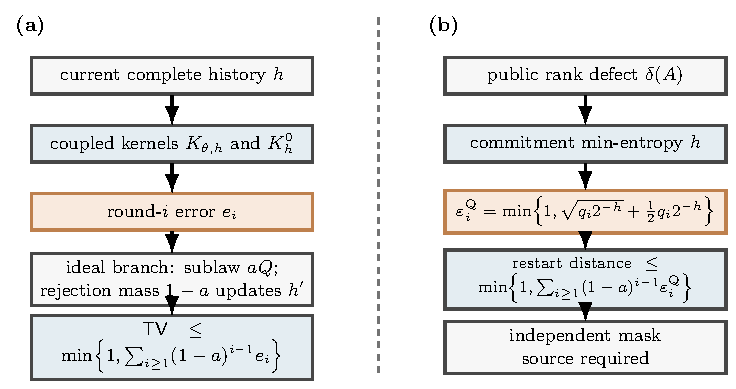
\includegraphics[width=.98\textwidth]{fig-retry-qrom.pdf}
\caption{Classical and QROM restart interfaces.  (a) At history $h$, the real
and ideal full-trial kernels are compared within $e_i$; only the ideal accepted
branch has sublaw $aQ$.  The restart hybrid weights the round-$i$ discrepancy
by the ideal survival probability $(1-a)^{i-1}$.  (b) The public rank defect
supplies commitment min-entropy $h$; $q_i$ bounds the prior quantum queries in
round $i$, adaptive reprogramming gives $\varepsilon_i^{\rm Q}$, and the same
survival weights control the restarted state.
The QROM branch requires an independent mask source and is not a reduction for
the complete ML-DSA signing algorithm.}
\label{fig:retry-qrom}
\end{figure}

\section{Public-rank and generating-function details}
\label{app:rank-details}

This resource derives the general rank--bucket bound, specializes it to the
public ML-DSA commitment map~\cite{FIPS204}, and records the finite-field rank generating
function used for the ideal-XOF tail.  The main text uses only the resulting
point-mass certificate.

\begin{theorem}[Rank--bucket fiber certificate]
\label{thm:rank-bucket}
Let $L:\mathbb F_q^D\to\mathbb F_q^K$ have rank $r$, let
$\Omega\subseteq\mathbb F_q^D$, and let each coordinate of a quantizer $Q$
have fibers of size at most $B$.  For every injective encoding $E$,
\begin{equation}
 \max_x|(E\circ Q\circ L)^{-1}(x)\cap\Omega|
 \le\min\{|\Omega|,B^rq^{D-r}\}.                    \label{eq:rank-bucket-uniform}
\end{equation}
Consequently a uniform $Y\in\Omega$ satisfies
\begin{equation}
 H_\infty(E(Q(LY)))\ge
 \log_2|\Omega|-\log_2\min\{|\Omega|,B^rq^{D-r}\}. \label{eq:rank-bucket-entropy}
\end{equation}
\end{theorem}

\begin{proof}
Choose $r$ independent output coordinates.  Fixing their quantized values
permits at most $B^r$ exact outputs, and each exact output has a kernel coset
of size $q^{D-r}$.  Intersect with $\Omega$ and take logarithms.
\end{proof}

For ML-DSA, $Y$ is uniform on $I_{\gamma_1}^{D}$ and the encoded commitment is
\begin{equation}
 g_{A,\mu}(y)=
 \mu\mathbin\|\woneEncode(\HighBits(Ay)).
 \label{eq:mldsa-commitment-map}
\end{equation}
For this map, write
$q=8380417$, $n=256$, $D=n\ell$, and let
$\widehat A[j]\in\mathbb F_q^{k\times\ell}$ be the public NTT lanes.  Define
\begin{equation}
 \delta(A)=\sum_{j=0}^{n-1}
 \bigl(\ell-\rank_{\mathbb F_q}\widehat A[j]\bigr).   \label{eq:mldsa-rank-defect}
\end{equation}

\begin{proposition}[ML-DSA commitment-fiber certificate]
\label{prop:mldsa-fiber}
Let $B_{\gamma_2}=2\gamma_2+1$.  For every public matrix $A$ and message
representative $\mu$, the largest fiber $M_{A,\mu}$ of
\eqref{eq:mldsa-commitment-map} and its min-entropy obey
\begin{align}
 M_{A,\mu}
 &\le\min\{(2\gamma_1)^D,
 B_{\gamma_2}^{D-\delta(A)}q^{\delta(A)}\},          \label{eq:mldsa-fiber-bound}\\
 h_{A,\mu}
 &\ge\max\left\{0,D\log_2\frac{2\gamma_1}{B_{\gamma_2}}
 -\delta(A)\log_2\frac q{B_{\gamma_2}}\right\}.    \label{eq:mldsa-entropy-bound}
\end{align}
The certificate is deterministic and checkable from the public key.
\end{proposition}

\begin{table}[ht]
\centering
\caption{Checklist for the ML-DSA commitment-fiber instantiation.}
\label{tab:mldsa-fiber-interfaces}
\small
\renewcommand{\arraystretch}{1.08}
\begin{tabularx}{\textwidth}{@{}>{\raggedright\arraybackslash}p{.19\textwidth}p{.34\textwidth}X@{}}
\toprule
Interface & Object used in the proof & Check \\
\midrule
mask embedding
 & $I_{\gamma_1}^{D}\hookrightarrow\mathbb F_q^D$
 & injective because $2\gamma_1<q$ \\
coefficient linear map
 & $L_A:R_q^\ell\to R_q^k$, $y\mapsto Ay$
 & an $\mathbb F_q$-linear map before \textsc{HighBits} \\
NTT rank transfer
 & $\mathcal N_kL_A\mathcal N_\ell^{-1}=\bigoplus_j\widehat A[j]$
 & $\mathcal N_\ell,\mathcal N_k$ are bijections, so ranks are equal \\
scalar quantizer
 & coefficientwise $\HighBits$
 & every bucket has at most $B_{\gamma_2}=2\gamma_2+1$ residues \\
protocol encoding
 & $\mu\|\woneEncode(\HighBits(Ay))$
 & fixed prefix and injective fixed-width encoding preserve fibers \\
\bottomrule
\end{tabularx}
\end{table}

\begin{proof}[Proof of Proposition~\ref{prop:mldsa-fiber}]
FIPS~204 has $2\gamma_2\mid q-1$.  Directly from its
\textsc{Decompose} exceptional branch, every \textsc{HighBits} value has
either $2\gamma_2$ or $2\gamma_2+1$ residue preimages; hence the maximum
bucket size is $B_{\gamma_2}$.  Let
$\mathcal N_\ell:R_q^\ell\to\mathbb F_q^{n\ell}$ and
$\mathcal N_k:R_q^k\to\mathbb F_q^{nk}$ be the vector NTT isomorphisms.  If
$L_A(y)=Ay$ is written in the coefficient basis, then the defining lane-wise
NTT multiplication gives the exact conjugacy
\begin{equation}
 \mathcal N_k\circ L_A\circ\mathcal N_\ell^{-1}
   =\bigoplus_{j=0}^{n-1}\widehat A[j].
   \label{eq:mldsa-ntt-conjugacy}
\end{equation}
The two outer maps are bijections.  Therefore rank invariance under
composition with isomorphisms and rank additivity for a direct sum give
\begin{align*}
 \rank_{\mathbb F_q}L_A
 &=\sum_{j=0}^{n-1}\rank_{\mathbb F_q}\widehat A[j]\\
 &=\sum_{j=0}^{n-1}\bigl(\ell-(\ell-\rank\widehat A[j])\bigr)
   =n\ell-\delta(A)=D-\delta(A).
\end{align*}
This equality concerns only the linear rank.  We now return to the coefficient
basis, where FIPS applies \textsc{HighBits} coefficientwise, and apply
Theorem~\ref{thm:rank-bucket} with the displayed rank and bucket bound.  The
mask interval embeds injectively in $R_q^\ell$ because $2\gamma_1<q$.
Finally, prepending the fixed $\mu$ and applying the injective fixed-width
\textsc{w1Encode} neither merge nor enlarge a fiber.  These five steps prove
\eqref{eq:mldsa-fiber-bound}; taking logarithms and clipping by the source size
proves~\eqref{eq:mldsa-entropy-bound}.
\end{proof}

\subsection*{Ideal-XOF defect distribution}

If
\begin{equation}
 \mathcal N_{k,\ell}(r)=
 \prod_{i=0}^{r-1}
 \frac{(q^k-q^i)(q^\ell-q^i)}{q^r-q^i}              \label{eq:finite-field-rank-count}
\end{equation}
denotes the number of rank-$r$ matrices in
$\mathbb F_q^{k\times\ell}$, then in the ideal-XOF model the total NTT-lane
defect has the exact probability generating function
\begin{equation}
 \E[X^\delta]=
 \left(\sum_{e=0}^{\ell}
 \frac{\mathcal N_{k,\ell}(\ell-e)}{q^{k\ell}}X^e\right)^n. \label{eq:defect-pgf}
\end{equation}
Indeed, the $n$ NTT lanes are independent uniform rectangular matrices.
Applying the standard finite-field rank count to each lane and multiplying the
one-lane generating functions proves~\eqref{eq:defect-pgf}.

\section{Scoped ML-DSA strict-\texorpdfstring{$z$}{z} illustration}
\label{app:mldsa-illustration}

As a deliberately scoped illustration of the interfaces above, consider only
the strict $z$ predicate of ML-DSA~\cite{FIPS204}.  Put $q=8380417$, $n=256$,
$D=n\ell$, $\beta=\tau\eta$, and $B_{\gamma_2}=2\gamma_2+1$.  With the public
NTT-rank defect $\delta(A)$ of~\eqref{eq:mldsa-rank-defect},
Proposition~\ref{prop:mldsa-fiber} bounds the commitment point mass by
\begin{equation}
 \epsilon_A:=
 \min\left\{1,
 \left(\frac{B_{\gamma_2}}{2\gamma_1}\right)^{D-\delta(A)}
 \left(\frac q{2\gamma_1}\right)^{\delta(A)}\right\}.
 \label{eq:mldsa-point-mass}
\end{equation}
The literal strict-$z$ common interval gives
\begin{equation}
 G_z=\left(\frac{2(\gamma_1-\beta)-1}{2\gamma_1}\right)^D.
 \label{eq:Afips}
\end{equation}
In the separated classical-oracle model,
Theorems~\ref{thm:rom-freshness} and~\ref{thm:retry-composition} yield,
for the counterfactual process that retries until this predicate alone
accepts,
\begin{equation}
 \TV_{\rm restart}\le
 \epsilon_A\left(\frac{q_0}{G_z}+\frac{1-G_z}{G_z^2}\right).
 \label{eq:mldsa-retry-bound}
\end{equation}

\begin{table}[ht]
\centering
\caption{Scoped ML-DSA strict-$z$ illustration in the separated classical
model with $q_0\le2^{64}$.  The budget is the largest rank defect for which
\eqref{eq:mldsa-retry-bound} is below $2^{-128}$; ACVP entries are audited
keys, not an all-key claim.}
\label{tab:mldsa-compact}
\small
\begin{tabular}{lrrrrrr}
\toprule
set & $D$ & $\beta$ & $\gamma_1$ & $G_z$ & defect budget & ACVP $\delta=0$\\
\midrule
ML-DSA-44 & 1024 & 78  & $2^{17}$ & .5414714311 & 51  & 25/25\\
ML-DSA-65 & 1280 & 196 & $2^{19}$ & .6188909137 & 272 & 25/25\\
ML-DSA-87 & 1792 & 120 & $2^{19}$ & .6623821841 & 400 & 25/25\\
\bottomrule
\end{tabular}
\end{table}

All 75 audited keys have zero defect; the corresponding restart exponents are
at least $128.578$, $129.109$, and $129.928$ bits.  This calculation concerns
only the strict $z$ predicate: it neither analyzes the conjunction of
Algorithm~7 filters nor constitutes a security reduction.

\bibliography{covariogram-balancing}

\end{document}
